%%%%%%%%%%%%
%
% $Autor: Wings $
% $Datum: 2019-03-05 08:03:15Z $
% $Pfad: ArduinoIDE.tex $
% $Version: 4250 $
% !TeX spellcheck = en_GB/de_DE
% !TeX encoding = utf8
% !TeX root = filename 
% !TeX TXS-program:bibliography = txs:///biber
%
%%%%%%%%%%%%


\chapter{Arduino IDE 2.3.x}


\ToDo{Citations\\
    Step by Step\\
Screen shots\\
First Steps}
    
    
\section{Overview of Arduino IDE}
	
	It is an open source official Arduino software which used for editing, uploading and compiling codes in to the Arduino module. It is a cross-platform software which is available for Operating Systems like Windows, Linux, macOS. It runs on Java platform and supports a range of Arduino modules. It supports C and C++ languages. The microcontrollers present on the Arduino boards are programmed which accepts the information in the form of code. The program written in the IDE is called a sketch which will generate a Hex file which is then transferred and uploaded in the controller. The IDE environment is made up of two parts: an editor and a compiler. The editor is used to write the required code, while the compiler is used to compile and upload the code to the Arduino Module. The Menu bar has options such as File in which there are many options including Opening a new file or existing, Examples-in which we can find sketches for different applications like Blink, Fade etc. There is an error console at the bottom of the screen for displaying errors.
	The 6 buttons are present on top of the screen are as follows:

		\begin{center}
		
\includegraphics[width=0.7\linewidth]{Arduino/ArdiunoIDE2/MenuButtons.png}
		\captionof{figure}{Menu Buttons}
	\end{center}
	
	
	\begin{itemize}
		\item The check mark is used to verify your code. Click this once you have written your code.
		\item The arrow uploads your code to the Arduino to run.
		\item The dotted paper will create a new file.
		\item The upward arrow is used to open an existing Arduino project.
		\item The downward arrow is used to save the current file.
		\item The far right button is a serial monitor, which is useful for sending data from the Arduino to the PC for debugging purposes.
	\end{itemize}
	
	
\section{Installation (MacOS)}
	
	To install the Arduino IDE, we need to download the latest version from the Arduino webpage \url{https://www.arduino.cc/en/software}. We can select the version based on the operating system we are using. Here we are installing Arduino 2.3.2 for a MacOS(Sonoma 14.4.1) operating system. The set up file name is \FILE{arduino-ide\_2.3.2\_macOS\_64bit.dmg} and the size of it is 1,93,600 KB. The file is in Zip format. If you use Safari it will be automatically extracted. If you use a different browser you may need to extract it manually. The most recent offline arduino IDE 2.3.2 can be seen in Figure ~\ref{fig:ArduinoIDE Create Agent Installation} it is also supportive for all operating systems.
	
		\begin{center}
			
			\includegraphics[width=0.7\linewidth]{Arduino/ArdiunoIDE2/ArduinoIdeCreateAgentInstallation.png}
			%\label{fig:ArduinoIDE Create Agent Installation}
			\captionof{figure}{ArduinoIDE Create Agent Installation}
			\label{fig:ArduinoIDE Create Agent Installation}
		\end{center}
		
		\begin{center}
			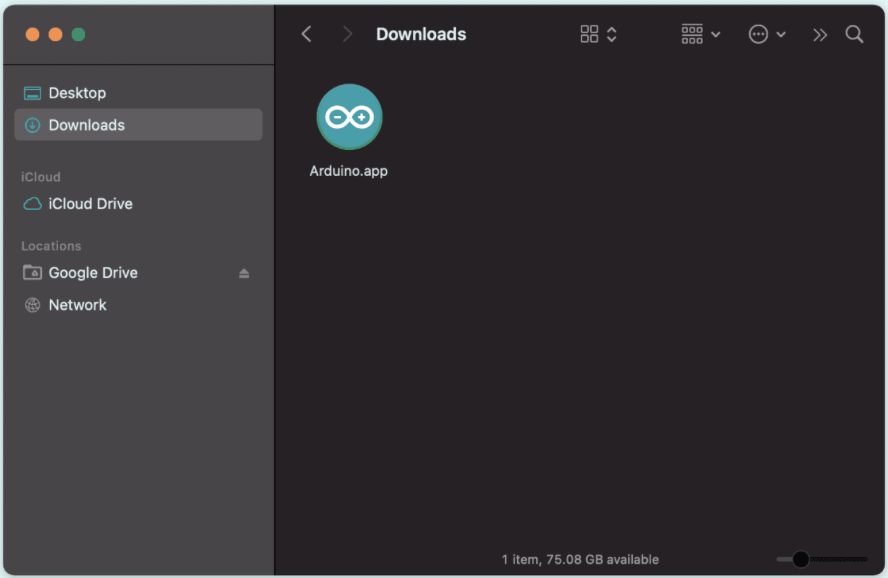
\includegraphics[width=0.7\linewidth]{Arduino/ArdiunoIDE2/OpenTheDownloadFolder.png}
			\captionof{figure}{Open the Downloadf folder}
		\end{center}
		
	Copy the Arduino application bundle into the Applications folder (or elsewhere on your computer) then it look like Figure \ref{fig:Copy to the Applications folder}
		
		\begin{center}
			
			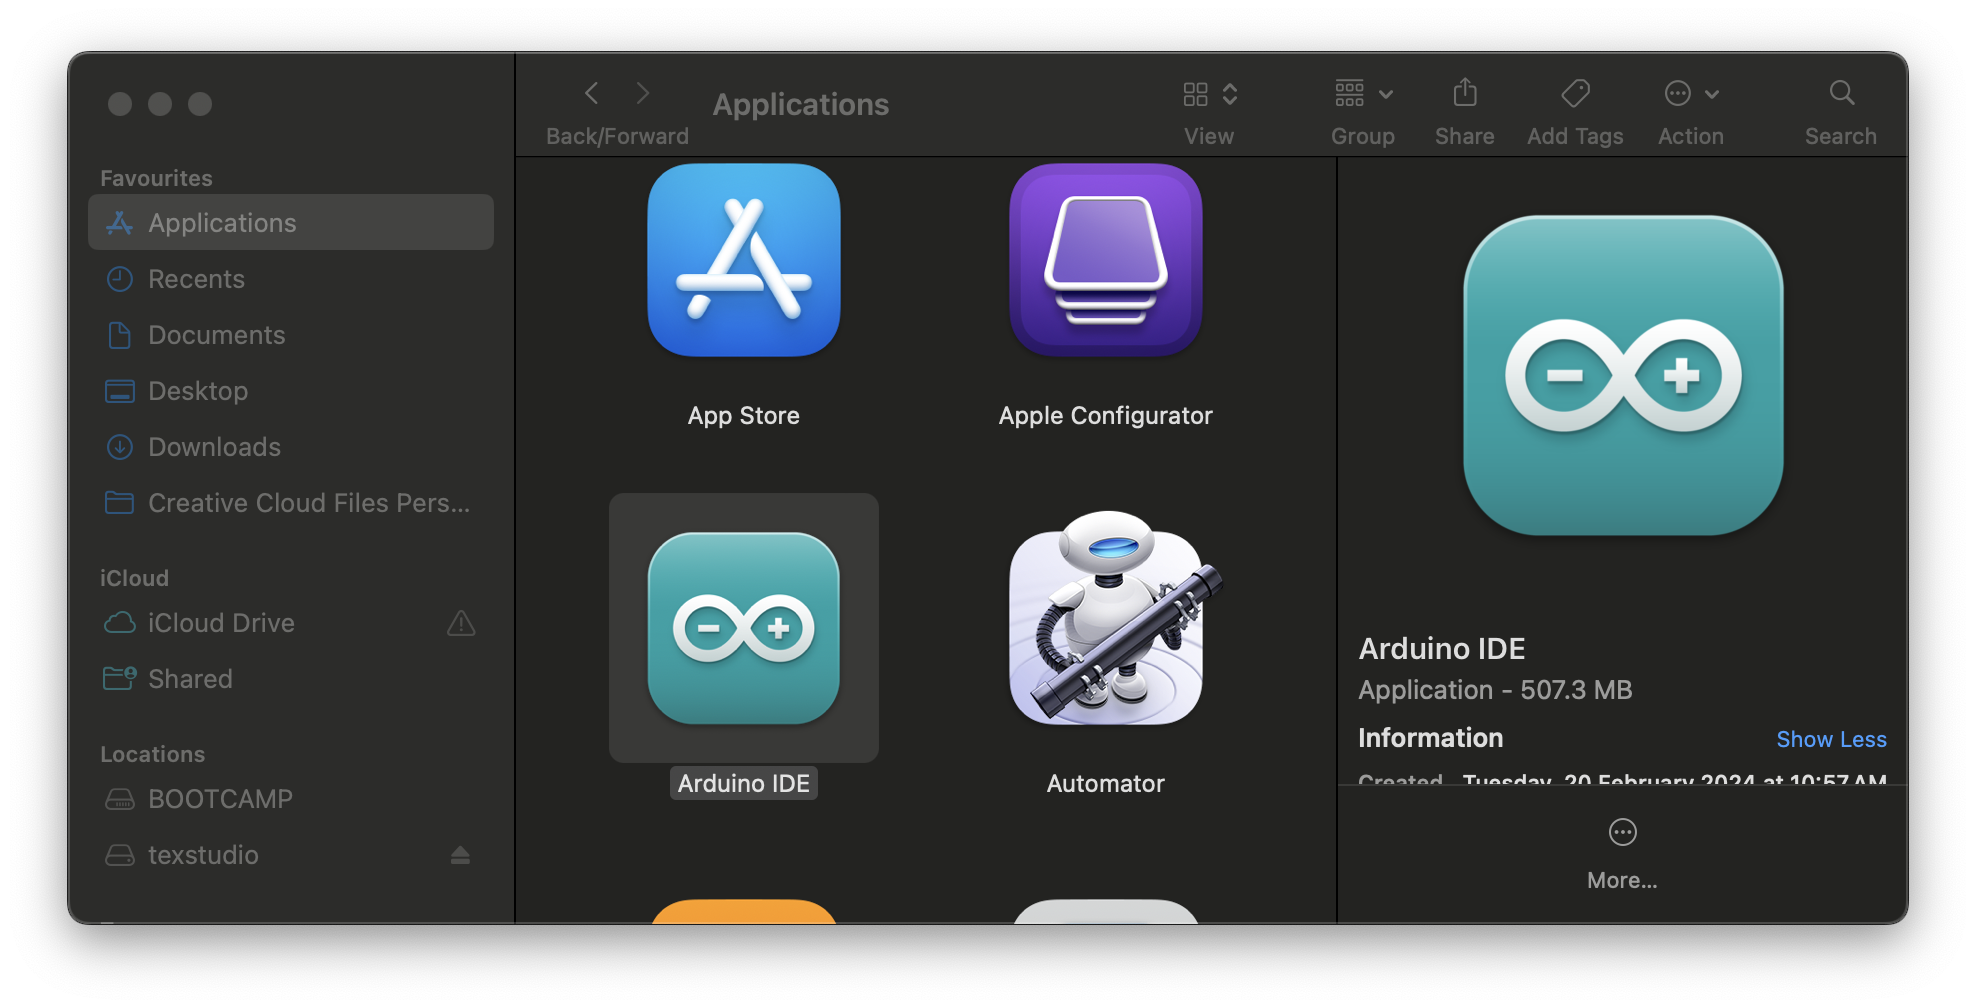
\includegraphics[width=0.7\linewidth]{Arduino/ArdiunoIDE2/CopyToTheApplicationsFolder.png}
			\label{fig:Copy to the Applications folder}
			\captionof{figure}{Copy to the Applications folder}
		\end{center}
		
	It can be seen from the Figure \ref{fig:Arduino Sketch} that the basic Arduino sketch has two parts. 
	
	\begin{itemize}
		\item Void setup(): This function returns void and we do the intiliaztion such as the output LED color, specifying the core etc
		\item Void loop(): In this function we define functions which are to be performed throughout the loop. These codes are placed between paranthesis {} and each function has a return type, here it has void return type.
	\end{itemize}
	
	\begin{center}
		\label{fig:Arduino Sketch}
		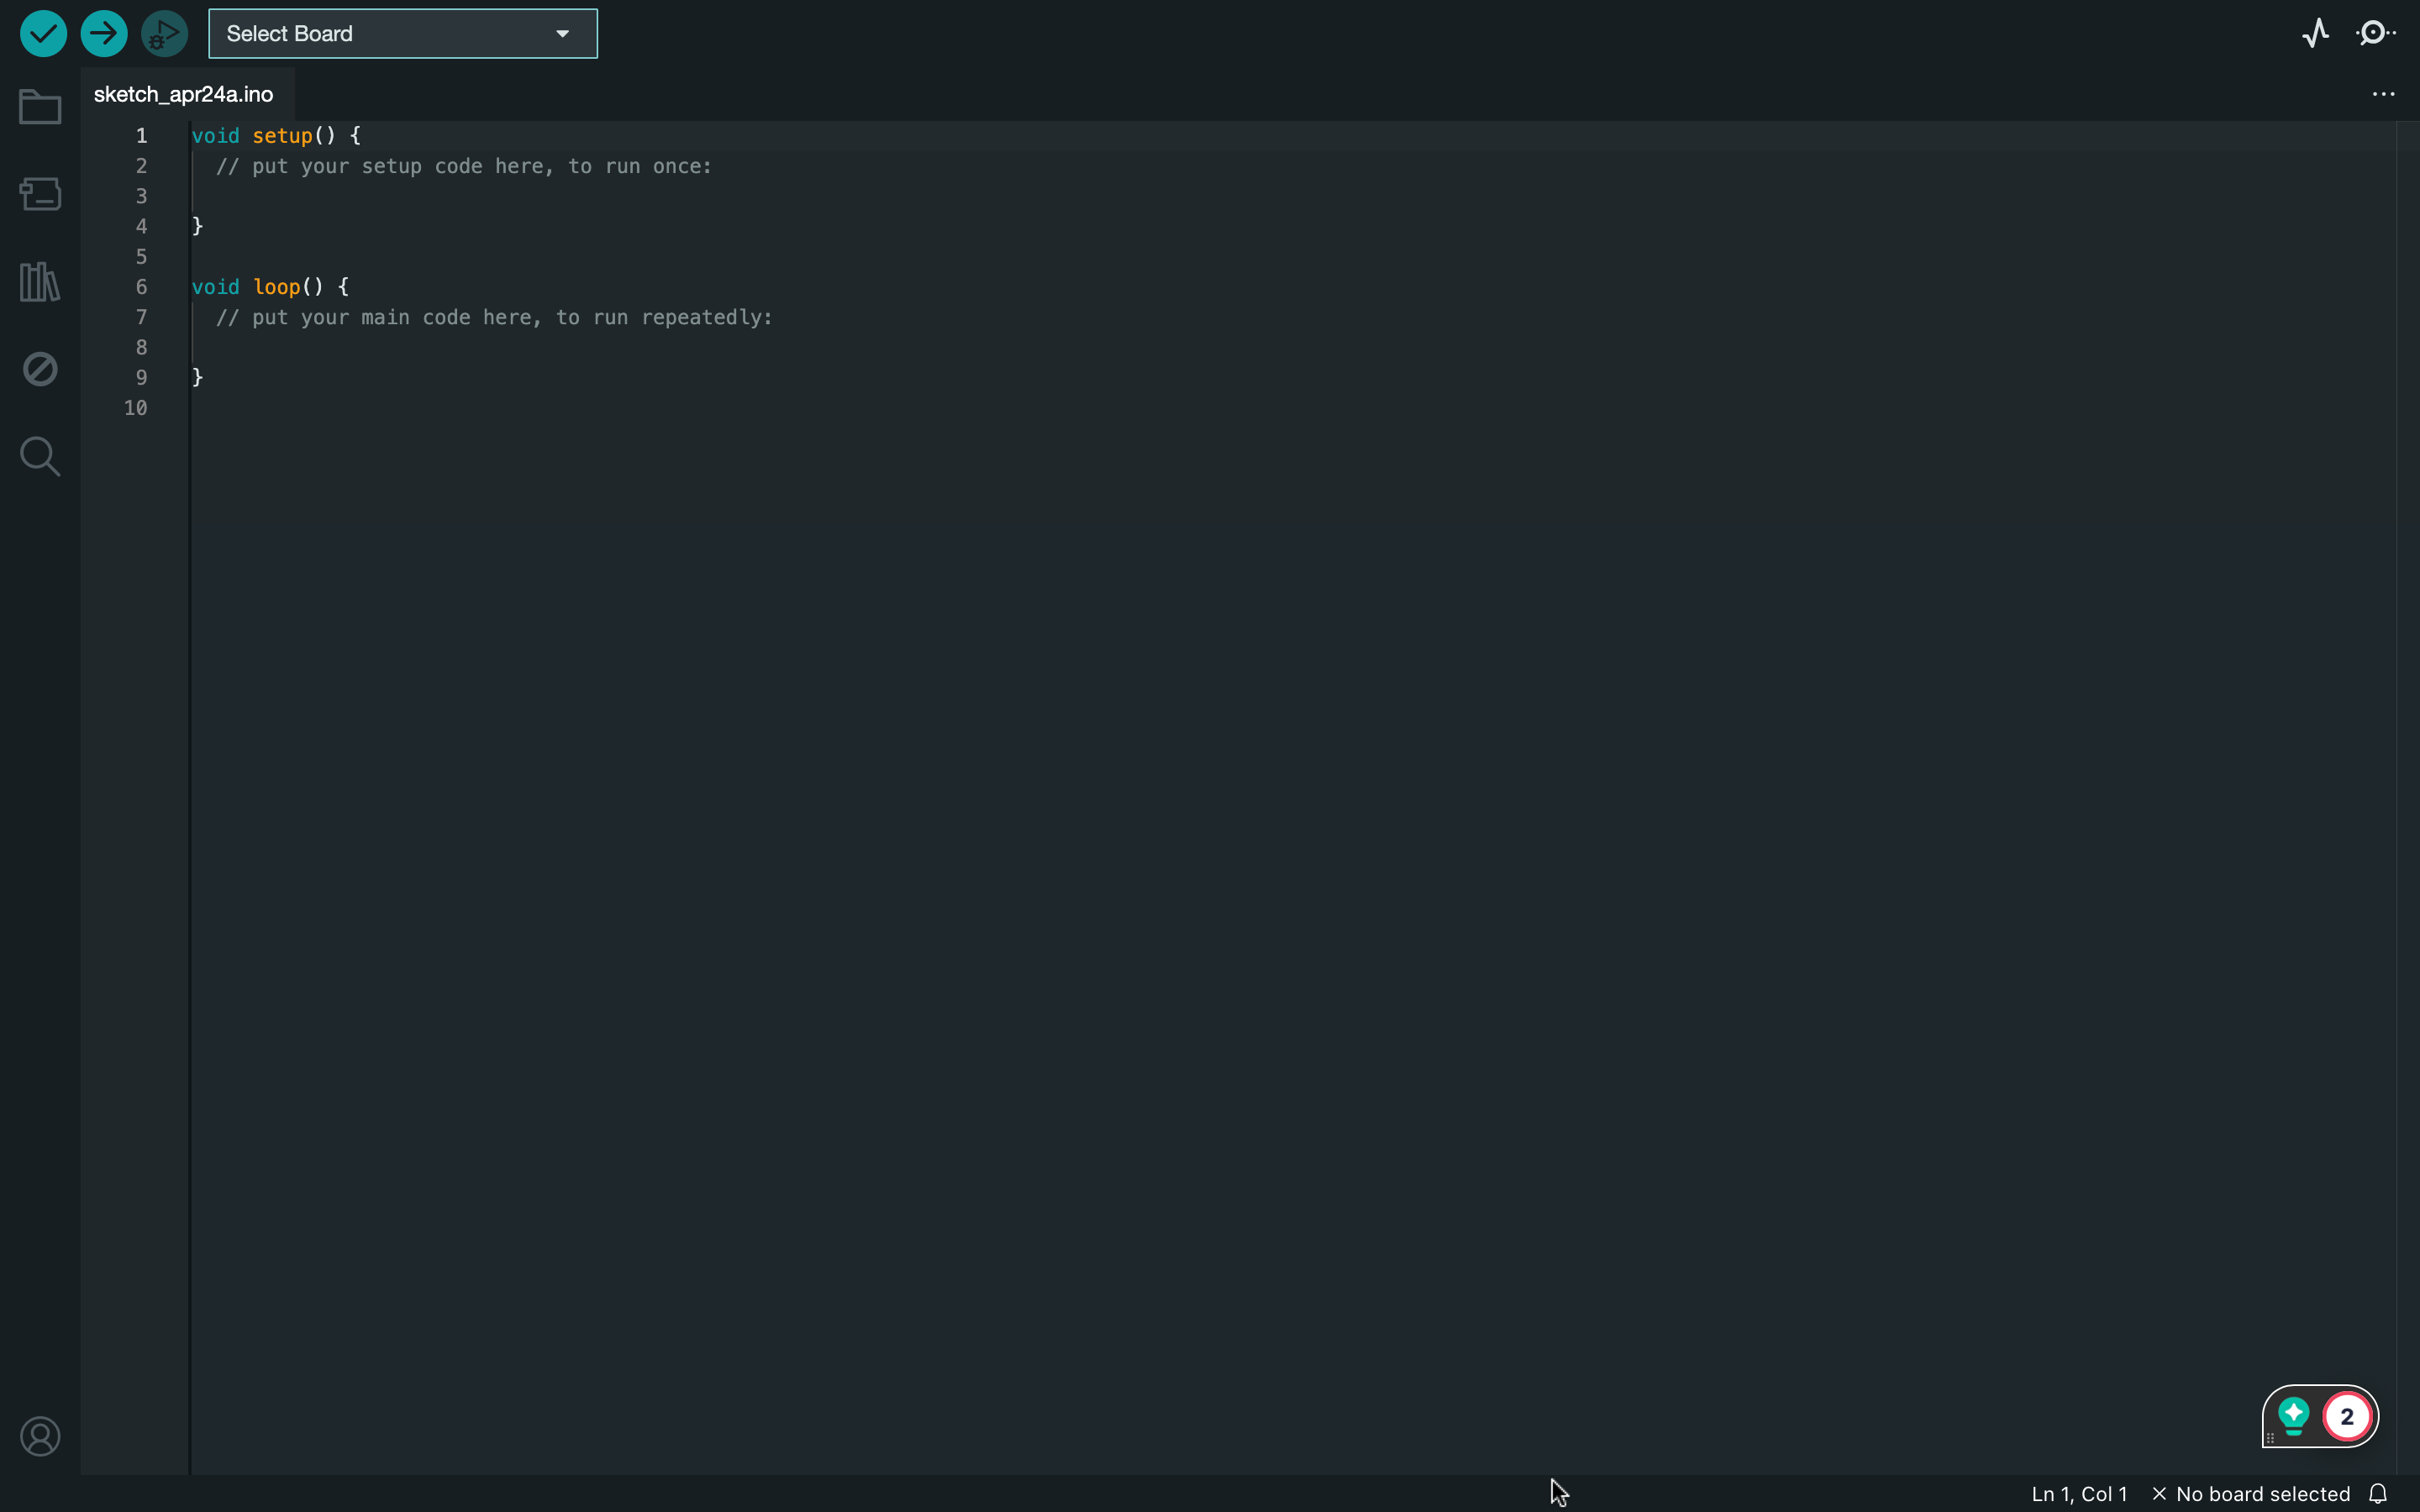
\includegraphics[width=0.7\linewidth]{Arduino/ArdiunoIDE2/ArduinoIDESketch2.png}
		\captionof{figure}{Arduino Sketch}
	\end{center}